\documentclass[paper=a4,11pt,titlepage,twoside=true,headings=normal,numbers=noenddot,captions=tableabove,listof=totoc,index=totoc,bibliography=totoc]{scrreprt}
%\usepackage{amsmath} % abgesetzte Formeln zentriert in der Zeile
%\usepackage[fleqn,intlimits]{amsmath} % [fleqn] abgesetzte Formeln mit festem Abstand zum linken Rand
\usepackage[reqno,intlimits]{amsmath} % [reqno] um die gleichungsnummerierung rechts zu haben
% intlimits: Grenzen für Integrale unterhalb und oberhalb des Zeichens
\usepackage{amssymb}
\usepackage{array}
\usepackage[ngerman]{babel}
\usepackage[ngerman]{varioref}
\usepackage[T1]{fontenc} 
\usepackage[utf8]{inputenc}
%---------------------------
\usepackage{booktabs}
\usepackage{calc}
\usepackage{cancel}
\usepackage[labelfont={footnotesize,sf,bf},textfont={footnotesize,sf}]{caption} %Format (Textgröße, Textform) für Bildtext 
%normalsize
%scriptsize
% sc --> smallcaps
% bf --> bold face
% sf --> sans serif
%\usepackage{cleveref} % löscht labels!!!!!!!!!!
%\usepackage{cite} %inkompatibel mit biblatex
\usepackage[table]{xcolor}
%\usepackage{colortbl}
\usepackage[right]{eurosym}
%\usepackage{caption2} %nicht zusammen mit sidecap
%\usepackage{exscale}
\usepackage{ellipsis}
\usepackage{graphicx}
\usepackage{float}
%\usepackage{floatflt}
%----------------------------------------
\usepackage{gensymb} %-----------
%\usepackage{helvet}
\usepackage{csquotes}
\usepackage{listings}
\usepackage{longtable}
\usepackage{lastpage}  %----------
\usepackage{lscape}
\usepackage{lmodern}  %-- Silbentrennung
%\usepackage{mathpazo} % andere mathematische Symbol
\usepackage{makeidx}
%\usepackage{minitoc}
\usepackage{multirow}
\usepackage{multicol}
%\usepackage[intoc]{nomencl}   % zwei Spalten beim Formelzeichenverzeichnis
\usepackage[german,intoc]{nomentbl} %vier Spalten bei Formelzeichenverzeichnis
\usepackage{nicefrac} %----
%\usepackage{picins} %----------
\usepackage{paralist} %--------
\usepackage{parallel}  %----------
\usepackage{pdfpages} %-------
% Define user colors using the RGB model
%\usepackage{colortbl}
%\definecolor{dunkelgrau}{rgb}{0.8,0.8,0.8}
%\definecolor{hellgrau}{rgb}{0.95,0.95,0.95}
%\usepackage{pgfplots}
\usepackage[figuresright]{rotating} 
\usepackage{scrlayer-scrpage}
%\usepackage[innercaption]{sidecap} %Beschriftung neben Bild, Tabelle, Mittelbach S333 %----------
\usepackage{sistyle}
% \usepackage[locale=DE]{siunitx} %nicht zusammen mit sistyle %---------
% \usepackage[locale=DE,per-mode=fraction,parse-numbers=false]{siunitx} %nicht zusammen mit sistyle %---------
% \usepackage[locale=DE,parse-numbers=false]{siunitx} %nicht zusammen mit sistyle %---------
\usepackage[font={scriptsize,sl},captionskip=3pt]{subfig} % für die Unterbilder %---------
\usepackage{shortvrb}
\usepackage{tablefootnote}
\usepackage{tabularx}
\usepackage{tabulary}
\usepackage{textcomp}
\usepackage{tocbasic}
%\usepackage{tikz}
\usepackage{times} 
\usepackage{units} %----------
\usepackage{url}
\usepackage{wrapfig} %----------
\usepackage{xr-hyper}
\usepackage{arydshln} %für \hdashline[5pt/2pt] % muss am Ende stehen, sonst gibt es Probleme mit xcolor
\usepackage{hyperref} % muss am Schluss stehen
\hypersetup{linkcolor={0 1 1}, linkbordercolor={1 1 1}, citebordercolor={1 1 1}} % setzt Linkboxen auf Farbe "`weiß"'
%\usepackage{bm}
%\usepackage[toc,symbols]{glossaries} %---------- muss nach hyperref stehen
\usepackage[nonumberlist, acronym, toc, section]{glossaries} % muss nach hypersetup stehen
%----------------
%\usepackage{romannum} % Seitenzahlen in römischen Ziffern
%\usepackage{adjustbox}
\usepackage{scrhack}
\usepackage[style=numeric, citestyle=numeric, backend=biber]{biblatex}
%-------------------------
 %\renewcommand{\captionlabelfont}{\sffamily} %für "Abbildung" und "Tabelle"
 %\renewcommand{\captionfont}{\sffamily\small} %für den Text der Bildunterschriften
%  \renewcommand{\captionlabelfont}{\sffamily} 
%  \renewcommand{\captionfont}{\sffamily} %\renewcommand{\normalfont}{\sffamily} %für die Überschriften
% Fettdruck der Bezeichnung Abbildung, Tabelle
%\renewcommand{\captionlabelfont}{\bfseries}
%---------------------------------------------
%------------------ Schrifttyp in der Kopf- und Fusszeilen
\setkomafont{pageheadfoot}{\footnotesize\sffamily}
%---------------------------------------------------
%Ändern der Abbildung- und Tabellenbezeichnung (Niedermair S.157)
%_____________________________________________
\addto\captionsngerman{\renewcommand\figurename{Abb.}}
\addto\captionsngerman{\renewcommand\tablename{Tab.}}
\renewcommand\listfigurename{Abbildungen}
%_______________________________
%Betrag eines Wertes
\newcommand{\abs}[1]{\lvert #1 \rvert} 
%---------------------------------------------
\newcommand{\absatz}[1]{\textbf{\textsc{#1}}} %siehe Mittelbach S. 876ff
%----------------------------
%\newcommand{\absatz}{\par \medskip}
%______________________________
%\newcommand{\anhang}[1]{Anhang \ref{#1}, Seite \pageref{#1}}
\newcommand{\anhang}[1]{Anhang \vref{#1}}
%________________________________
\newcommand{\aufgabe}{\stepcounter{plus} Aufgabe \arabic{plus}}
%______________________________________
%compactitem
\newcommand{\bci}{\begin{compactitem}}
\newcommand{\eci}{\end{compactitem}}
%______________________________________
%
\newcommand{\bi}{\begin{itemize}}
\newcommand{\ei}{\end{itemize}}
%______________________________________
%compactenumerate
\newcommand{\bce}{\begin{compactenum}}
\newcommand{\ece}{\end{compactenum}}
%_____________________________________
%begin equation
\newcommand{\be}{\begin{equation}}
\newcommand{\ee}{\end{equation}}
%_____________________________________
%begin equation ohne Formelnummer
\newcommand{\ben}{\begin{equation*}}
\newcommand{\een}{\end{equation*}}
%_____________________________________
%begin align ohne Formelnummer
\newcommand{\ban}{\begin{align*}}
\newcommand{\ean}{\end{align*}}
%_____________________________________
%begin align
\newcommand{\ba}{\begin{align} }
\newcommand{\ea}{\end{align}}
%_____________________________________
%minpage
\newcommand{\bmp}{\begin{minipage}[t]{.47\linewidth}}
\newcommand{\emp}{\end{minipage}}
%_____________________________
%  dB
\newcommand{\db}{dB}
%  dB(A)
\newcommand{\dba}{ dB(A) }
%  dB(A) für Satzende
\newcommand{\dbap}{ dB(A)}
%_________________________________
\newcommand{\bzw}{bzw.\,}
%_______________________________
\newcommand{\dif}{\mathrm{d}}
%________________________________
% neuer Zähler
\newcounter{plus}
\setcounter{plus}{0}
%______________________________
%Für das Formelverzeichnis _____________________ Formelverzeichis ____
% Befehl umbenennen in fz
\let\fz\nomenclature
% Deutsche Überschrift
\renewcommand{\nomname}{Formelzeichen}
% Punkte zw. Abkürzung und Erklärung
\setlength{\nomlabelwidth}{.20\hsize}
\renewcommand{\nomlabel}[1]{#1 \dotfill}
% Zeilenabstände verkleinern
\setlength{\nomitemsep}{-\parsep}
%_____________________________
\newcommand{\bild}[1]{Abb. \vref{#1}}
\newcommand{\sbild}[1]{siehe Abb. \vref{#1}}
\newcommand{\bilder}[2]{Abb. \vrefrange{#1}{#2}}
\newcommand{\bildseite}[1]{Abb. \vref{#1}} % erzeugt "`Abb. nn auf Seite nn
\newcommand{\tabelle}[1]{Tab. \vref{#1}}
\newcommand{\tabellenseite}[1]{Tab. \vref{#1}} % erzeugt "`Tab. nn auf Seite nn
% für \vref ist usepackage[german]{varioref} einzufügen
%_-------------------------------- Freiraum
\newcommand{\freiraum}[1]{\begin{figure}[H]\vspace{#1\textheight}\end{figure}}
%_____________________________
% Gleichung
\newcommand{\gl}[1]{Gl.\,(\ref{#1})}
\newcommand{\sgl}[1]{siehe Gl.\,(\ref{#1})}
\newcommand{\glbereich}[2]{Gl. \vrefrange[]{#1}{#2}}
%_____________________________
% Grad Celsius
\newcommand{\grad}{\,\degC}
\newcommand{\gradC}{\,\degree}
%______________________________________
% Großbuchstaben als Indizes kleiner schreiben; spezielle im Mathemodus
\newcommand{\klein}[1]{\scriptscriptstyle{#1}}% Fettdruck der Bezeichnung 
%______________________________
%% Kasten
\newcommand{\kasten}{\fbox{\rule{0.0pt}{10pt}{{ } } }}
%______________________________
%\newcommand{\kapitel}[1]{Kapitel \ref{#1}, Seite \pageref{#1}}
\newcommand{\kapitel}[1]{Kapitel \vref{#1}}
%_____________________________
%  LAeq für den äquivalenten Dauerschallpegel
\newcommand{\laeq}{ $L_{Aeq}$ }
%  LAeq für den äquivalenten Dauerschallpegel am Satzende
\newcommand{\laeqp}{ $L_{Aeq}$}
%_________________________________
%   Linie zeichnen
\newcommand{\linie}{\rule{0.5\textwidth}{0.1pt}}
%---------------------- LaTeX
\newcommand{\lt}{\LaTeX\,\,}
%----------------------------
\newcommand{\nl}{\newline}
%__________________________________
%  multicolumn für Tabellen
\newcommand{\mc}{\multicolumn}
%% \mc{1}{c}{Text}
%_________________________________
%    Parallel
\newcommand{\pl}[1]{\ParallelLText{#1}}
\newcommand{\pr}[1]{\ParallelRText{#1}}
\newcommand{\pp}{\ParallelPar}
%------------ rot unterstrichen
\newcommand{\rotunterstrichen}[1]{\textcolor{red}{\underline{\textcolor{black}{#1}}}}
%________________ Realteil
\newcommand{\real}[1]{\text{Re}\left\{#1\right\}}
%________________________________--
\newcommand{\seite}[1]{Seite \pageref{#1}}
\newcommand{\seiten}[2]{\vpagerefrange{#1}{#2}}
%----------------------------
%        TEXT Rot
\newcommand{\textrot}[1]{\textcolor{red}{#1}}
%______________________________
%Abkürzung für \multicolumn
\newcommand{\tab}[2]{\multicolumn{1}{#1}{#2}}
%_____________________________________
% doppelt unterstreichen
\newcommand{\unterstreichen}[1]{\underline{\underline{#1}}}
% einfach unterstreichen
\newcommand{\ul}[1]{\underline{#1}}
%______________________________
%kurze Verbatimausgabe
%\MakeShortVerb{\|} %mittelbach S.160 mit \usepackage{shortvrb}
%_______________________________________
% vspace
\newcommand{\vsf}{\vspace{5pt}}
%_________________________________
\newcommand{\zb}{z.B.\,}
\newcommand{\idr}{i.d.R.\,}
%_______________________________
% Zähler-einfach
\newcounter{req}
\newcommand{\zaehler}[1]{\refstepcounter{req}{#1} \thereq}
%% Beispielaufzählung \zaehler{Beispiel}\\
%_____________________________________
 \setlength{\voffset}{-2.532 cm}
 \setlength{\hoffset}{-1.57 cm}
% \setlength{\topmargin}{2.0 cm} \setlength{\topskip}{0.1 cm}
 \setlength{\topmargin}{1.5 cm}
 \setlength{\topskip}{0.1 cm}
 \setlength{\evensidemargin}{1.5 cm}
 \setlength{\oddsidemargin}{1.5 cm}
 \setlength{\textwidth}{16.5 cm}
 \setlength{\footskip}{40pt}
 \setlength{\textheight}{24.5cm}
% \setlength{\textheight}{23.5 cm}
 \setcounter{page}{1}
 \setlength{\parindent}{0cm}
 \setlength{\headsep}{20pt}
%----------------------------------------------------------------------
% Linien in der Kopf- und Fußzeile
%\renewcommand{\headrulewidth}{0.0pt}   %Linie in der Kopfzeile mit 0.0pt keine Linie
%%\renewcommand{\footrulewidth}{0.0pt}   %Linie in der Fußzeile mit 0.0 pt keine Linie
%\renewcommand{\headrulewidth}{0.2pt}   %Linie in der Kopfzeile mit 0.0pt keine Linie
%\renewcommand{\footrulewidth}{0.2pt}   %Linie in der Fußzeile mit 0.0 pt keine Linie
%------------------------------------------------------------------------
%\renewcommand{\normalfont}{\sffamily} %für die Überschriften
%\renewcommand{\chaptermark}[1]{\markboth{\chaptername\ \thechapter #1}{}}
%\renewcommand{\sectionmark}[1]{\markright{\thesection\ #1}}
% \rfoot{\leftmark\\\rightmark}

%Definitionen für Kopfzeile
% bei documentclass {report} hat der Eintrag für die [gerade Seite] keine Wirkung
%-------------------------------------------------------------
%%
%Einstellungen für Kopf- und Fusszeilen mit dem KOMA-Skript und \usepackage{scrpage2}
\pagestyle{scrheadings}
%\pagestyle{scrplain}
% le --> links, gerade Seite
% ce --> mittig, gerade Seite
% re --> rechts, gerade Seite
% lo --> links, ungerade Seite
% co --> mittig, ungerade Seite
% ro --> rechts, ungerade Seite
%---------------------------------------------
% Löschen aller Einträge
%\clearscrheadings
% \automark[section]{subsection}
% \pagemark --> Seitenzahl
% \automark --> Kapitelüberschriften
% \leftmark --> ??
% \rightmark --> ??
%::::::::::::::::::::::::::::::::::: Kopfzeile
% Kopfzeile gerade Seite
\automark[chapter]{chapter}
\lehead[]{\titelkopfzeilelinkseven}
\cehead[]{\titelkopfzeilemitteeven}
\rehead[]{\titelkopfzeilerechtseven}
% Kopfzeile ungerade Seite
\lohead[]{\titelkopfzeilelinksodd}
\cohead[]{\titelkopfzeilemitteodd}
\rohead[]{\titelkopfzeilerechtsodd}
% Linie in der Kopfzeile
%\setheadtopline{0.2pt} % obere Linie in der Kopfzeile; nur bei scrartcl
\setheadsepline{0.4pt} % untere Linie in der Kopfzeile; nur bei scrartcl
% Linie in der Fusszeile
%::::::::::::::::::::::::::::::::::: Fußzeile
% Fusszeile gerade Seite[plain-style]{scrheadings-style}
\lefoot[]{\titelfusszeilelinkseven} 
\cefoot[]{\titelfusszeilemitteeven}
\refoot[]{\titelfusszeilerechtseven}
% Fusszeile ungerade Seite
\lofoot[]{\titelfusszeilelinksodd}
\cofoot[]{\titelfusszeilemitteodd}
\rofoot[]{\titelfusszeilerechtsodd}
%\rofoot[\thepage ]{\thepage}
%\setfoottopline{0.2pt} % obere Linie in der Kopfzeile; nur bei scrartcl
\setfootsepline{0.4pt} % untere Linie in der Kopfzeile; nur bei scrartcl

% le --> links, gerade Seite
% ce --> mittig, gerade Seite
% re --> rechts, gerade Seite
% lo --> links, ungerade Seite
% co --> mittig, ungerade Seite
% ro --> rechts, ungerade Seite
% even --> gerade Seite
% odd --> ungerade Seite
%----------------------------------------- Kopfzeilentext
 \newcommand{\titelkopfzeilemitteeven}{}
 \newcommand{\titelkopfzeilemitteodd}{}
 \newcommand{\titelkopfzeilelinkseven}{Hochschule RheinMain}
 \newcommand{\titelkopfzeilelinksodd}{}
 \newcommand{\titelkopfzeilerechtseven}{}
 \newcommand{\titelkopfzeilerechtsodd}{Hochschule RheinMain}
 %----------------------------------------- Fußzeilentext
 \newcommand{\titelfusszeilemitteeven}{}
 \newcommand{\titelfusszeilemitteodd}{}
 \newcommand{\titelfusszeilerechtseven}{Studienbereich Angewandte Physik \& Medizintechnik}
 \newcommand{\titelfusszeilerechtsodd}{\thepage \hspace{0.5mm} von \pageref{LastPage}}
 \newcommand{\titelfusszeilelinkseven}{\thepage \hspace{0.5mm} von \pageref{LastPage}}
 \newcommand{\titelfusszeilelinksodd}{Studienbereich Angewandte Physik \& Medizintechnik}
\newcommand{\titelLV}{Physikalisches Praktikum 2}
%---------------------------- VARIABLEN festlegen ------------------
%----------- Pro Versuch zu ändernde Angaben -----------------------
\newcommand{\versuch}{3} % Versuchsnummer einfügen
\newcommand{\untertitelb}{Variabler Kondensator} % Titel des Versuchs einfügen
\newcommand{\datumLV}{27.10.2020} % Datum einfügen
\newcommand{\deadline}{10.11.2020} % Datum einfügen
%----------- TITEL
\newcommand{\untertitela}{Versuch P2-4}
% -------- Student 1
\newcommand{\nameA}{Herr Cihan Ünlü}
% --------- Student 2
\newcommand{\nameB}{Herr Dennis Hunter}
% --------- Student 3, falls vorhanden
\newcommand{\nameC}{Herr Student drei}
%::::::::::::::::::::::::::::::::::
%\input{chapters/glossar}
\addbibresource{quellen.bib}
\begin{document}
%-----------------------------------------------------------------
\begin{titlepage} 
	\newcommand{\HRule}{\rule{\linewidth}{0.5mm}} 	
	\centering
	\textsc{\Large Hochschule RheinMain \\
		
\includegraphics[width=0.15\textwidth]{logo-hsrm}\\[1cm]}
%	\textsc{\Large Hochschule RheinMain}\\[1cm]
	\textsc{\LARGE \titelLV}\\[0.5cm]
		\HRule\\[0.4cm]
	{\huge\bfseries \untertitela}\\[0.4cm] % Title des Dokuments
	{\huge\bfseries \untertitelb}\\[0.4cm] % Title des Dokuments
		\HRule\\[1.5cm]
%-------------------
%\begin{flushleft}
	\begin{minipage}{0.4\textwidth}
%	\begin{flushleft}
%\centering
		\large
		\textit{\underline{Autoren}}\\[0.5cm]
		\textsc{\nameA}\\[0.5cm]
		\textsc{\nameB}\\[0.5cm]
		%\textsc{\nameC}\\[0.5cm] 
%	\end{flushleft}
\end{minipage}
%------------------------------------
\vfill\vfill\vfill 
\textsc{\Large Fachbereich Ingenieurwissenschaften}\\[0.5cm]
\textsc{\large Studienbereich Angewandte Physik \& Medizintechnik}\\[0.5cm] 
\vfill	
Datum des Versuchs:\hspace{0.4cm} {\large\datumLV}\\
Abgabedatum:\hspace{0.4cm} {\large\deadline} 
\end{titlepage}

%-----------------------------------------------------
\tableofcontents
\newpage
%--------------------
\chapter{Einleitung}
%Ziel des Versuchs.
\section{Kapazität des variablen Kondensators}
Allgemein ist die Kapazität eines Kondensators durch \gl{eq:cap} definiert. Für den Fall eines Plattenkondensators dessen
Platten einen runden Querschnitt besitzen und parallel zueinander stehen lässt sich seine Kapazität vereinfacht durch
\gl{eq:plattencap} ausdrücken.
\begin{equation}
    C = \frac{Q}{U}
    \label{eq:cap}
\end{equation}
%
\begin{figure}[h]
    \centering
    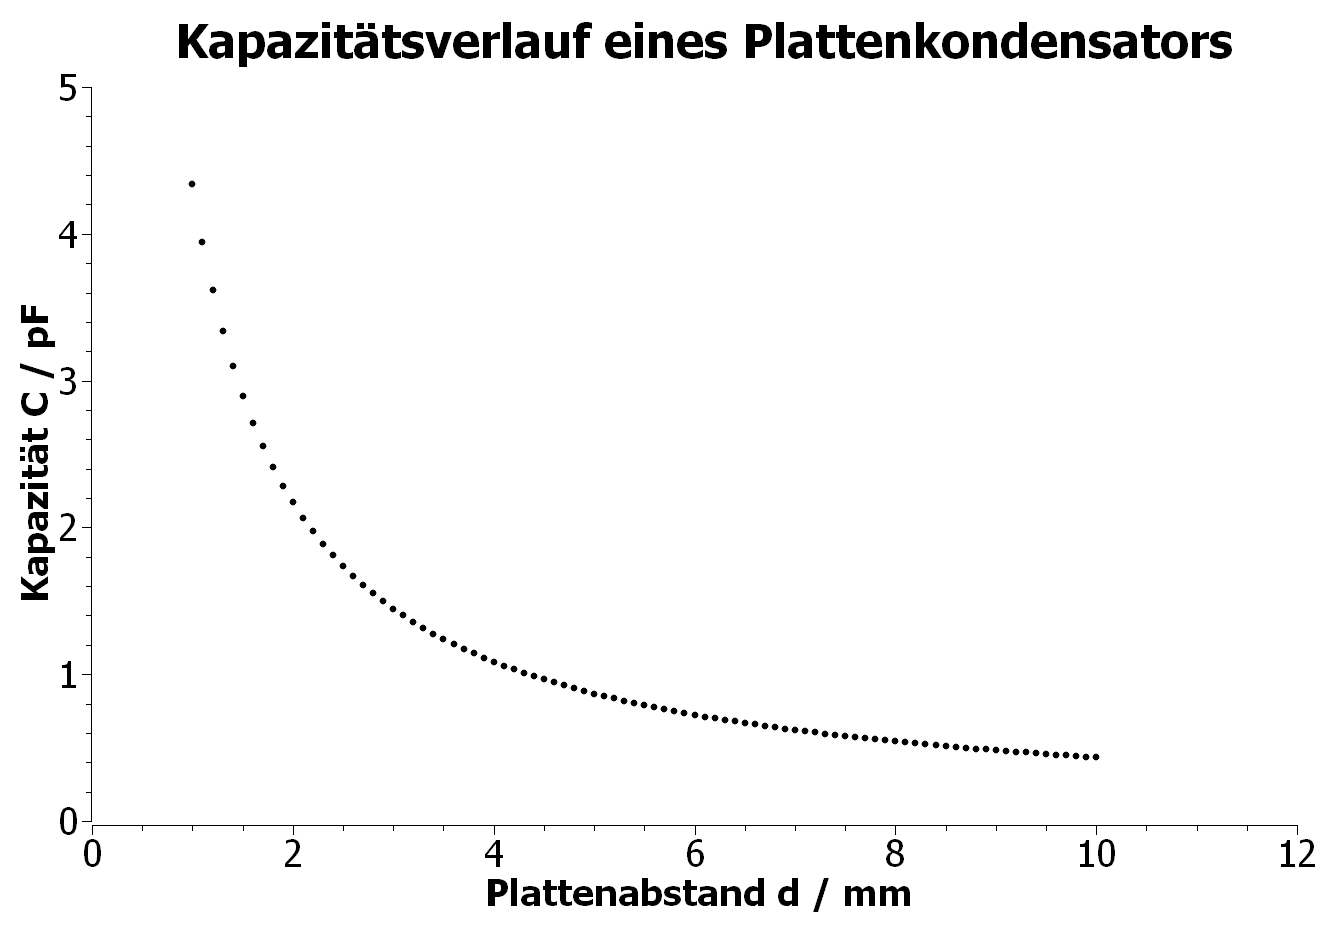
\includegraphics[width=.8\textwidth]{scidavis/kapazitaetsverlauf.jpeg}
    \caption[Kapazitätsverlauf eines Plattenkondensators]{Kapazitätsverlauf eines Plattenkondensators bei variablem Plattenabstand im Intervall \(\SI{1}{mm} \leq d \leq \SI{10}{mm}\)}
    \label{fig:kapVerlauf}
\end{figure}
%
\begin{equation}
    C = \varepsilon_0\varepsilon_r \cdot \frac{A}{d} \quad \text{und} \quad A = \frac{D^2 \pi}{4}
    \label{eq:plattencap}
\end{equation}
Hierbei ist \(\varepsilon_0\) die \textit{elektrische Feldkonstante} mit \(8,85 \cdot 10^{-12}\SI{}{\tfrac{As}{Vm}}\) \cite{Haberle.2007}
und \(\varepsilon_r\) die materialabhängige relative Permittivitätszahl. \bild{fig:kapVerlauf} zeigt den Kapazitätsverlauf
eines runden Plattenkondensators mit konstantem Durchmesser \(D = \SI{255}{mm}\), Luft als Dielektrikum (\(\varepsilon_r = 1\))
und einem Plattenabstand im Intervall \(\SI{1}{mm} \leq d \leq \SI{10}{mm}\). Es ist erkennbar, dass sich die Kapazität des Kondensators
bei größerem Plattenabstand rasch verringert und im weiteren Verlauf asymptotisch gegen \(0\) läuft.
%
%======================================================================================
%
\section{Bestimmung der Feldkonstante}
In die Form \(C_1(d^{-1}) = \varepsilon_0\varepsilon_r A \cdot d^{-1}\) gebracht lässt sich aus der Steigung des
linearisierten Kapazitätsverlaufs die Feldkonstante \(\varepsilon_0\) bestimmen.
\begin{figure}[h]
    \centering
    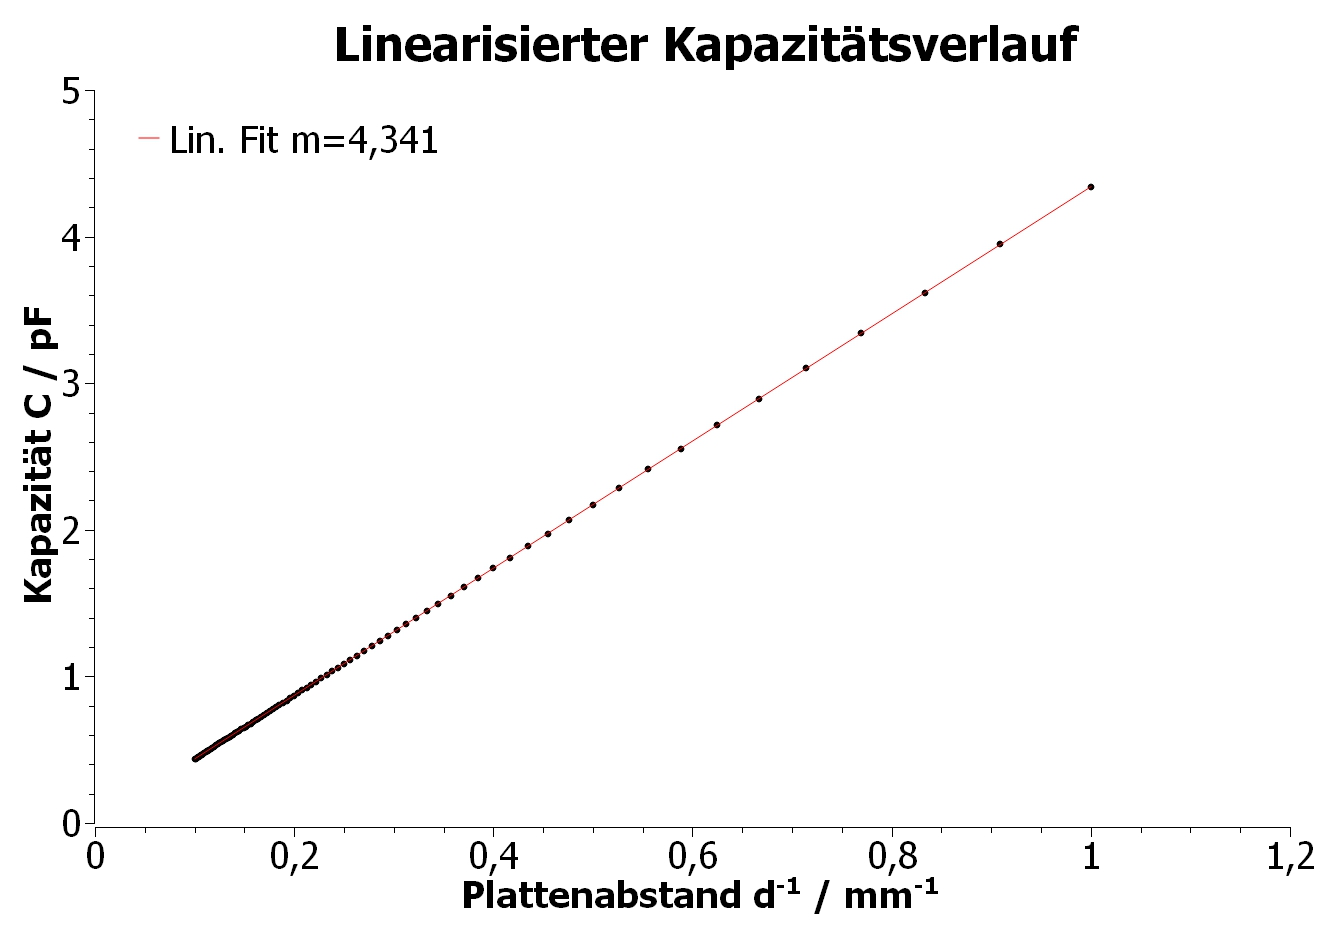
\includegraphics[width=.8\textwidth]{scidavis/linearisierter_kapazitaetsverlauf.jpeg}
    \caption[Linearisierter Kapazitätsverlauf]{Linearisierter Kapazitätsverlauf aus \bild{fig:kapVerlauf}. Mit bekannter Steigung der Ausgleichgeraden lässt sich die Feldkonstante \(\varepsilon_0\) bestimmen.}
    \label{fig:lin_kapVerlauf}
\end{figure}
\begin{align}
    m &= \varepsilon_0\varepsilon_r A \nonumber \\
    &\Leftrightarrow \nonumber \\
    \varepsilon_0 &= \frac{m}{\varepsilon_r A}
    \label{eq:e0}
\end{align}
%
%======================================================================================
%
\section{Bestimmung der Kapazität}
%
Die unbekannte Kapazität eines Kondensators \(C_1\) lässt sich mit einem einfachen Aufbau bestimmen. Der Kondensator
\(C_1\) wird an einer Konstantspannungsquelle zunächst auf eine definierte Spannung \(U_1\) geladen (siehe \bild{fig:c1laden}).
Im Gleichgewichtszustand beträgt die in \(C_1\) gespeicherte Ladung nach \gl{eq:cap}
\begin{equation}
    Q = C_1 \cdot U_1
    \label{eq:ladungc1}
\end{equation}
\begin{figure}[h]
    \centering
    \begin{minipage}[b]{.45\linewidth}
        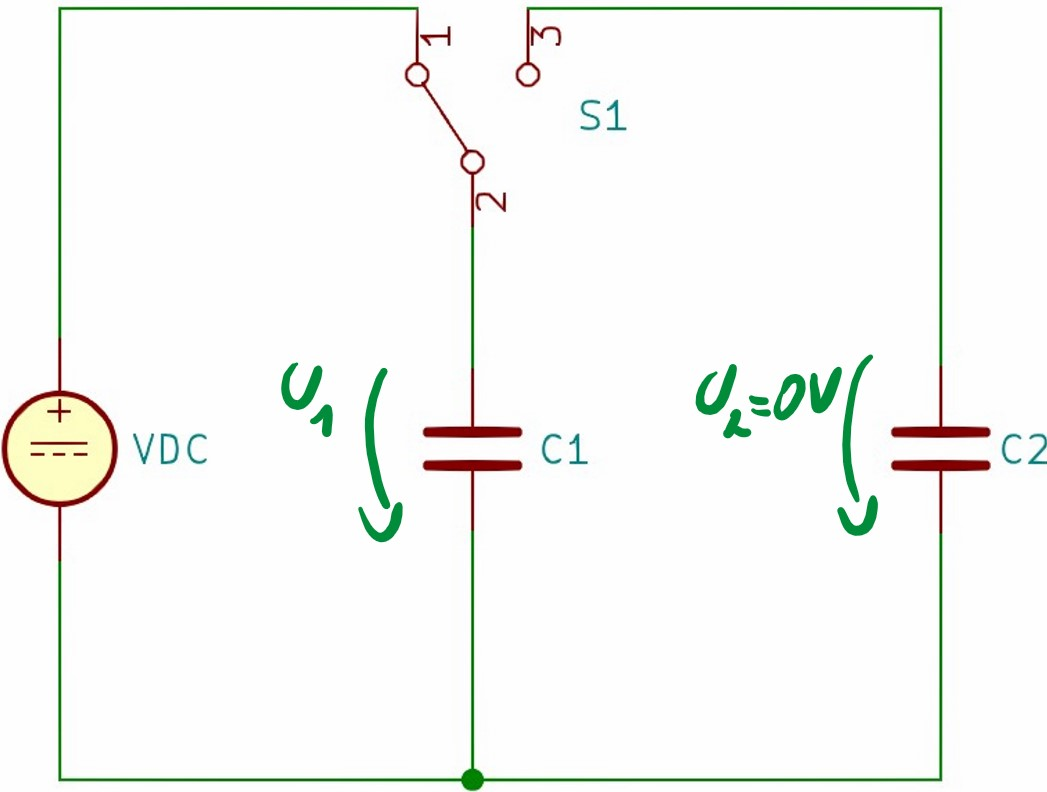
\includegraphics[width=.95\linewidth]{kicad/abbildungen/c1laden_annot.jpg}
        \caption[]{Initiales Laden des Kondensators \(C_1\).}
        \label{fig:c1laden}
    \end{minipage}
    \begin{minipage}[b]{.45\linewidth}
        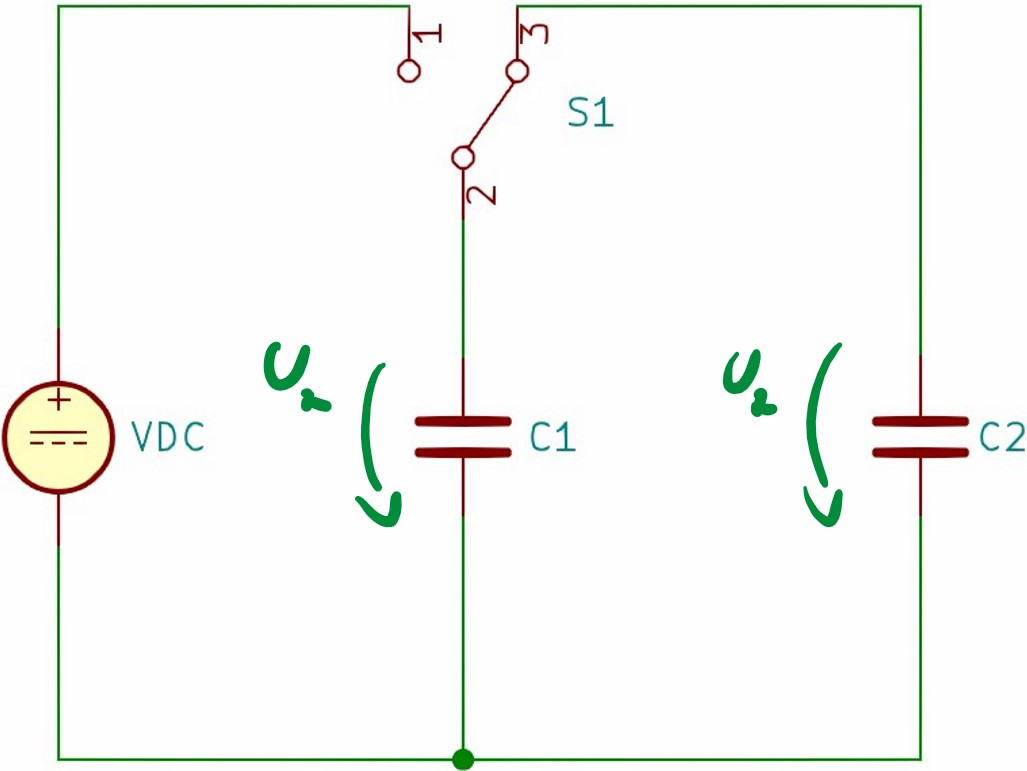
\includegraphics[width=.95\linewidth]{kicad/abbildungen/c1entladen_annot.jpg}
        \caption[]{Ladungsumverteilung von \(C_1\) hin zu \(C_2\).}
        \label{fig:c1entladen}
    \end{minipage}
\end{figure}
Wird nun \(S1\) umgeschaltet verteilt sich die in ihm gespeicherte Ladung \(Q\) um auf den nun parallel geschalteten,
anfangs vollständig entladenen Kondensator bekannter Kapazität \(C_2\). Die im System gespeicherte Gesamtladung \(Q\) bleibt
bei diesem Prozess erhalten. Für die Teilladungen gilt also
\begin{equation}
    Q = Q_1 + Q_2
    \label{eq:gesamtladung}
\end{equation}
Nachdem sich erneut ein Gleichgewicht eingestellt hat kann die nun an \(C_1\) wie \(C_2\) anliegende Spannung \(U_2 = \frac{Q_2}{C_2}\) gemessen
werden (vgl. \bild{fig:c1entladen}). Mit diesem Wissen und einsetzen von \gl{eq:ladungc1} in \gl{eq:gesamtladung} kann die Kapazität von \(C_1\) berechnet werden.
\begin{align}
    Q               &= Q_1 + Q_2 \nonumber \\
    C_1 \cdot U_1   &= C_1 \cdot U_2 + C_2 \cdot U_2 \nonumber \\
    \Leftrightarrow \quad C_1 (U_1 - U_2)                               &= C_2 \cdot U_2 \nonumber \\
    \Leftrightarrow \quad C_1                                           &= C_2 \cdot \frac{U_2}{U_1 - U_2}
    \label{eq:c1}
\end{align}
%
%==========================================================================
%
\section{Bestimmung der Dielektrizitätszahl}
Im Fall des Plattenkondensators unter Vernachlässigung von Effekten nahe der Plattenränder kann die elektrische Feldstärke
vereinfacht durch \gl{eq:feldPlatte} \cite{Halliday.2005} dargestellt werden.
\begin{equation}
    E = \frac{Q}{\varepsilon_0\varepsilon_r A}
    \label{eq:feldPlatte}
\end{equation}
Das Integral entlang der Feldlinien gibt die Potentialdifferenz oder die Spannung \(U\). Es folgt mit \gl{eq:feldPlatte}:
\begin{align}
    \int_{0}^{d} E \,\mathrm{d}s &= U = \frac{Q d}{\varepsilon_0\varepsilon_r A} \\
    &\Leftrightarrow \nonumber \\
    \frac{Q}{U} &= C = \varepsilon_0 \varepsilon_r \frac{A}{d}
    \label{eq:feldPlatte2}
\end{align}
Wird die Dielektrizitätszahl \(\varepsilon_r\) eines unbekannten Materials gesucht, kann jemand sich die Zusammenhänge
aus \gl{eq:feldPlatte2} zu Nutze machen.\par
Es sei der Raum zwischen den Platten eines Kondensators bekannter Plattenfläche \(A\), Kapazität \(C_0\) und Plattenabstand \(d\)
anfangs vollständig mit Luft gefüllt - für Luft kann \(\varepsilon_r = 1\) angenommen werden. Der Kondensator wird auf
eine Spannung geladen und im geladenen Zustand elektrisch isoliert.\par
Wird nun ein Dielektrikum zwischen die Platten des Kondensators Flächendeckend platziert, kann ein absinken der
Kondensatorspannung um den Faktor \(\varepsilon_r^{-1}\) fest gestellt werden. Da auch hier die im System gespeicherte Ladung
konstant bleibt geht damit nach \gl{eq:cap} eine Erhöhung der Kapazität einher. Die Dielektrizitätszahl des Materials
kann nun durch Vergleich der beiden Kapazitäten berechnet werden:
\begin{align}
    \frac{C_D}{C_0} &= \frac{\varepsilon_0\varepsilon_r \frac{A}{d}}{\varepsilon_0\varepsilon_{r,Luft} \frac{A}{d}} \nonumber \\
    \varepsilon_r &= \frac{C_D}{C_0} \cdot \varepsilon_{r,Luft} \nonumber \\
    &\Leftrightarrow \nonumber \\
    \varepsilon_r = \frac{C_D}{C_0} \quad &\text{für} \quad \varepsilon_{r,Luft} = 1
    \label{eq:rel_feld}
\end{align}

%\section{Gleichungen und Herleitungen}
%Herleitung der gegebenen Gl. aus den Grundgleichungen.

\chapter{Versuchsaufbau}
%
\begin{figure}[h]
    \centering
    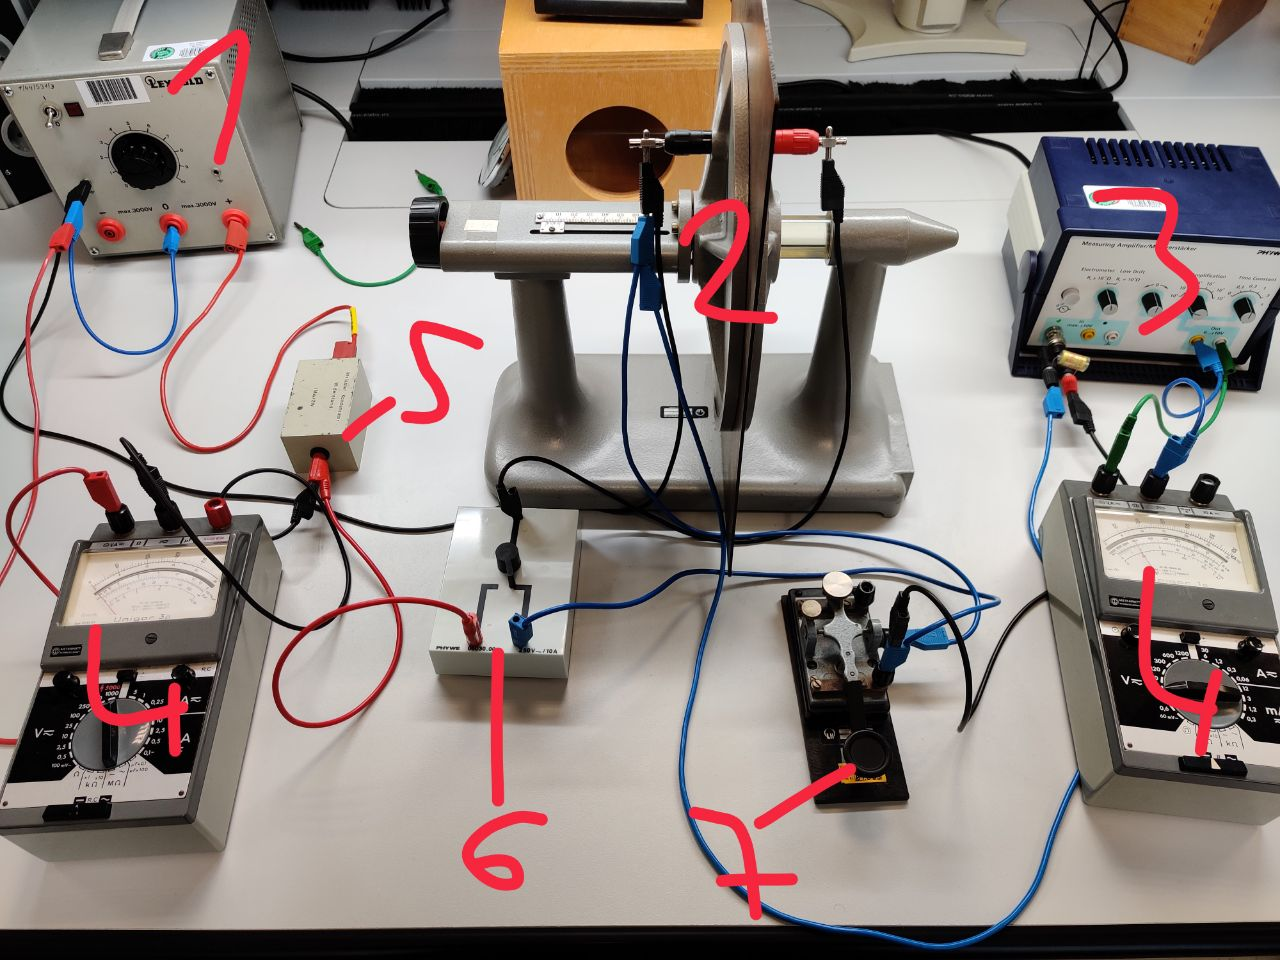
\includegraphics[width=\textwidth]{versuchsaufbau.jpg}
    \caption[Versuchsaufbau]{Versuchsaufbau mit variablem Kondensator und komplementären Geräten.
    1: Hochspannungsnetzteil,
    2: Variabler Kondensator $ C_{1} $ (links: geerdete Platte, rechts: isolierte Platte) mit Dielektrikum,
    3: Messverstärker des Herstellers \textit{PHYWE} mit Vergleichskondensator $ C_{2}=\SI{220}{nF}\cdot(1\pm10\%) $,
    4: Spannungsmessgerät (\textit{Unigor 3} zur Messung von $ U_{1} $, \textit{Unigor 1} zur Messung von $ U_{2} $),
    5: Vorwiderstand $ \SI{1}{M\ohm} $ im Gehäuse,
    6: Umschalter,
    7: Taster.
    }
    \label{fig:aufbau}
\end{figure}
%
\section{Messprinzip}
Das Hochspannungsnetzteil lädt den Kondensator $ C_{1} $ auf während das Messgerät die Spannung $ U_{1} $ misst.
Wird die Schaltung umgeschaltet, so entlädt der Vergleichskondensator $ C_{2} $ den ersten Kondensator $ C_{1} $. Die
dadurch verringerte Spannung wird vom zweiten Messgerät über den Messverstärker registriert. Wird der Umschalter wieder
betätigt, so lädt sich der Kondensator $ C_{1} $ wieder auf. Bedient man den Taster, dann entlädt sich der Kondensator
$ C_{2} $. Über das Verstellrad kann der Abstand $ d $ der Platten variiert und mit der Skala abgelesen werden.
\begin{figure}[h]
    \centering
    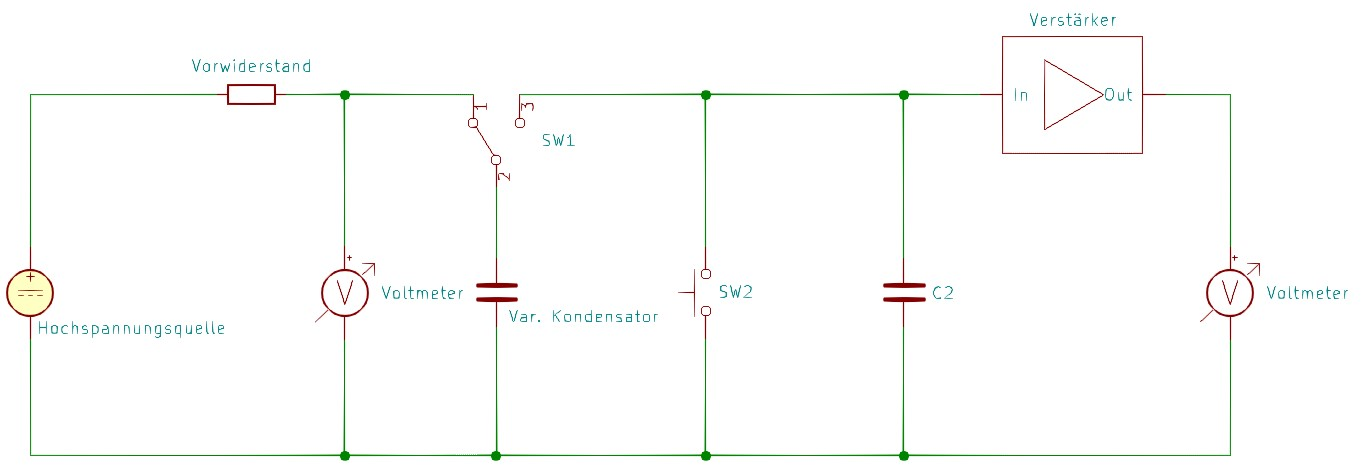
\includegraphics[width=\textwidth]{kicad/abbildungen/aufbau.jpg}
    \caption[Schaltskizze des Messaufbaus]{Schaltskizze des Messaufbaus.}
    \label{fig:schematic_aufbau}
\end{figure}
\input{chapters/4_durchführung}
\chapter{Auswertung}
\section{Kapazität des variablen Kondensators}
Durch \gl{eq:c1} lässt sich die Kapazität $ C_{1} $ des Kondensators in Abhängigkeit der Kapazität des Vergleichskondensators $ C_{2}=\SI{220}{nF}$
und den beiden Spannungen $ U_1 $ und $ U_2(d) $
der Messtabelle \tabelle{tab:mess1} berechnen.\par
\gl{eq:plattencap} gibt uns den eigentlich berechneten Wert der Kapazität $ C_{1} $ mit $\varepsilon_{0}=\SI{8,854}{\cdot 10^{-12}\frac{As}{Vm}}$,
$ \varepsilon_{R,Luft}=1 $ und $ D=\SI{0,255}{m} $ für $ \SI{1}{mm} \leq d \leq \SI{10}{mm} $.\par
Trägt man die drei experimentell bestimmten Kapazitäten zusammen mit der berechneten als Funktion des Abstandes auf, so erhält man
folgendes Diagramm:\par
\begin{figure}[h]
    \centering
    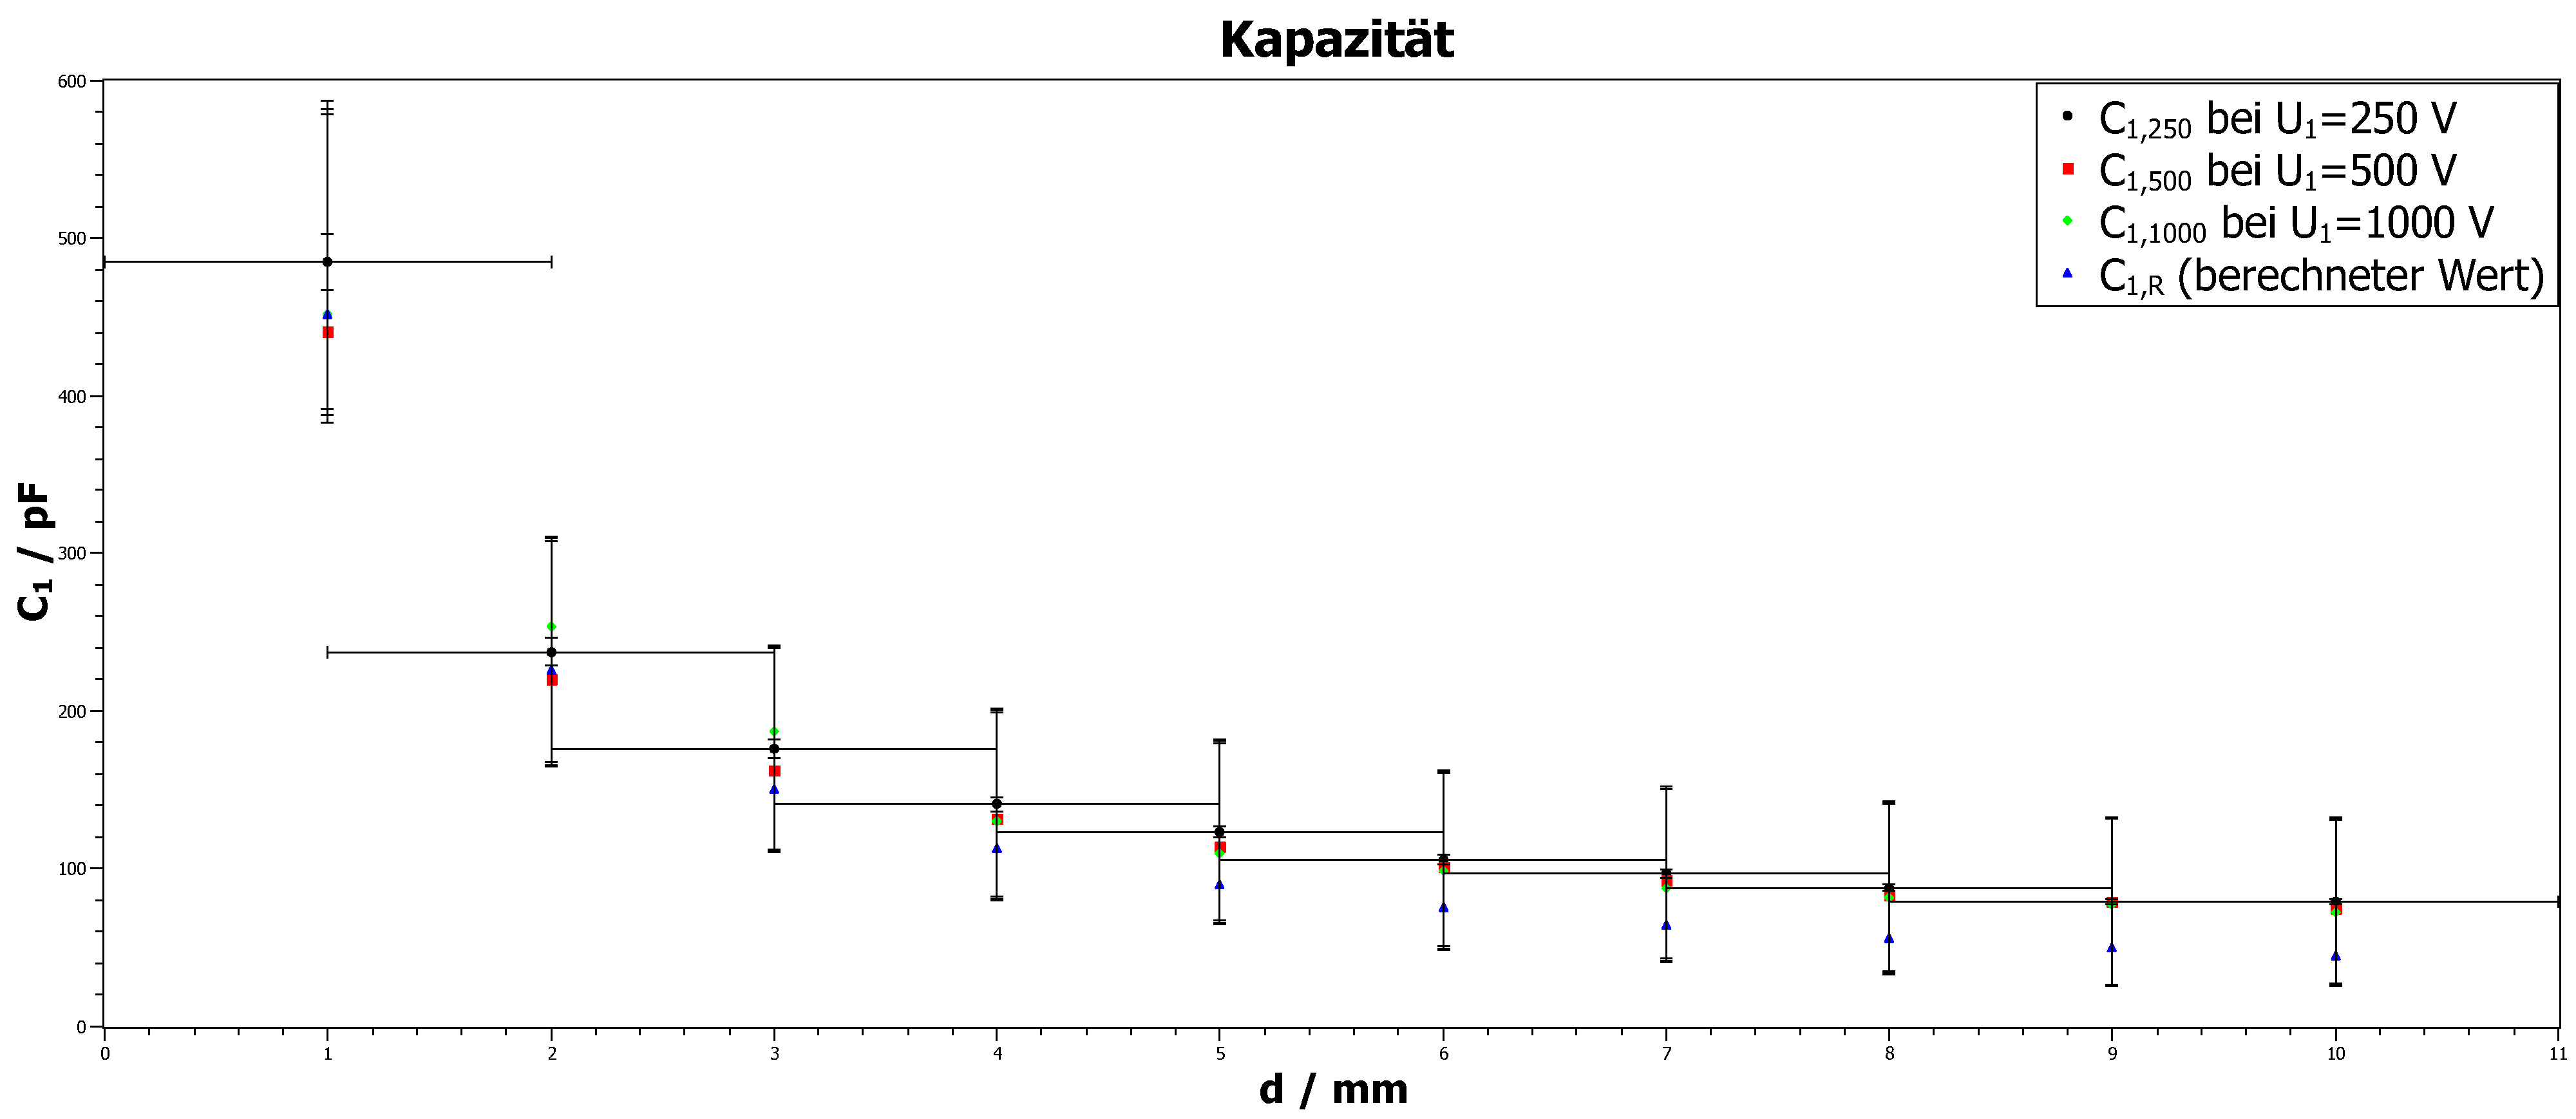
\includegraphics[width=.95\textwidth]{diagramme/Kapazitaet.pdf}
    \caption[Diagram Kapazität]{Diagram Kapazität}
    \label{fig:farad}
\end{figure}
%
\subsection{Fehler der experimentell bestimmten Kapazität}
Für den Fehler der experimentell bestimmten Kapazitäten gilt:
\begin{align}
    C_{1} &= C_{2}\cdot \left(\frac{U_{1}}{U_{2}}-1\right)^{-1} \nonumber \\
    \Delta C_{1} &= \left\vert\frac{\partial C_{1}}{\partial C_{2}}\right\vert\cdot \Delta C_{2} + \left\vert\frac{\partial C_{1}}{\partial U_{1}}\right\vert\cdot \Delta U_{1} + \left\vert\frac{\partial C_{1}}{\partial U_{2}}\right\vert\cdot \Delta U_{2} \nonumber \\
    &= \left(\frac{U_{1}}{U_{2}}-1\right)^{-1}\cdot \Delta C_{2} + C_{2}\cdot\left(\frac{U_{1}}{U_{2}}-1\right)^{-2}\cdot \frac{1}{U_{2}}\cdot\Delta U_{1} + C_{2}\cdot\left(\frac{U_{1}}{U_{2}}-1\right)^{-2}\cdot \frac{U_{1}}{U_{2}^{2}}\cdot\Delta U_{2}
\end{align}
Für den Fehler der berechneten Kapazität gilt:
\begin{align}
    C_{1,R} &= \varepsilon_{0} \varepsilon_{R} \cdot \frac{D^{2} \pi}{4 d} \nonumber \\
    \Delta C_{1,R} &= \left\vert\frac{\partial C_{1,R}}{\partial D}\right\vert\cdot \Delta D + \left\vert\frac{\partial C_{1,R}}{\partial d}\right\vert\cdot \Delta d \nonumber \\
    &= \varepsilon_{0}\varepsilon_{R}\cdot\frac{D \pi}{2 d}\cdot \Delta D + \varepsilon_{0} \varepsilon_{R}\cdot\frac{D^{2} \pi}{4 d^{2}}\cdot \Delta d
\end{align}
mit $ \Delta D= \SI{0,005}{m} $
%
%
%
\section{Bestimmung der elektrischen Feldkonstante}
Über die Steigung $ m $ der Ausgleichsgeraden der Funktion $ C_{1}(d^{-1}) $ lässt sich mittels \gl{eq:e0} die
elektrische Feldkonstante $\varepsilon_0$ bestimmen. Wird $ C_{1,\SI{1000}{V}} $ über $ d^{-1} $ aufgetragen ergibt sich
der in \bild{fig:mu_0} zu sehende Verlauf\par
\begin{figure}[h]
    \centering
    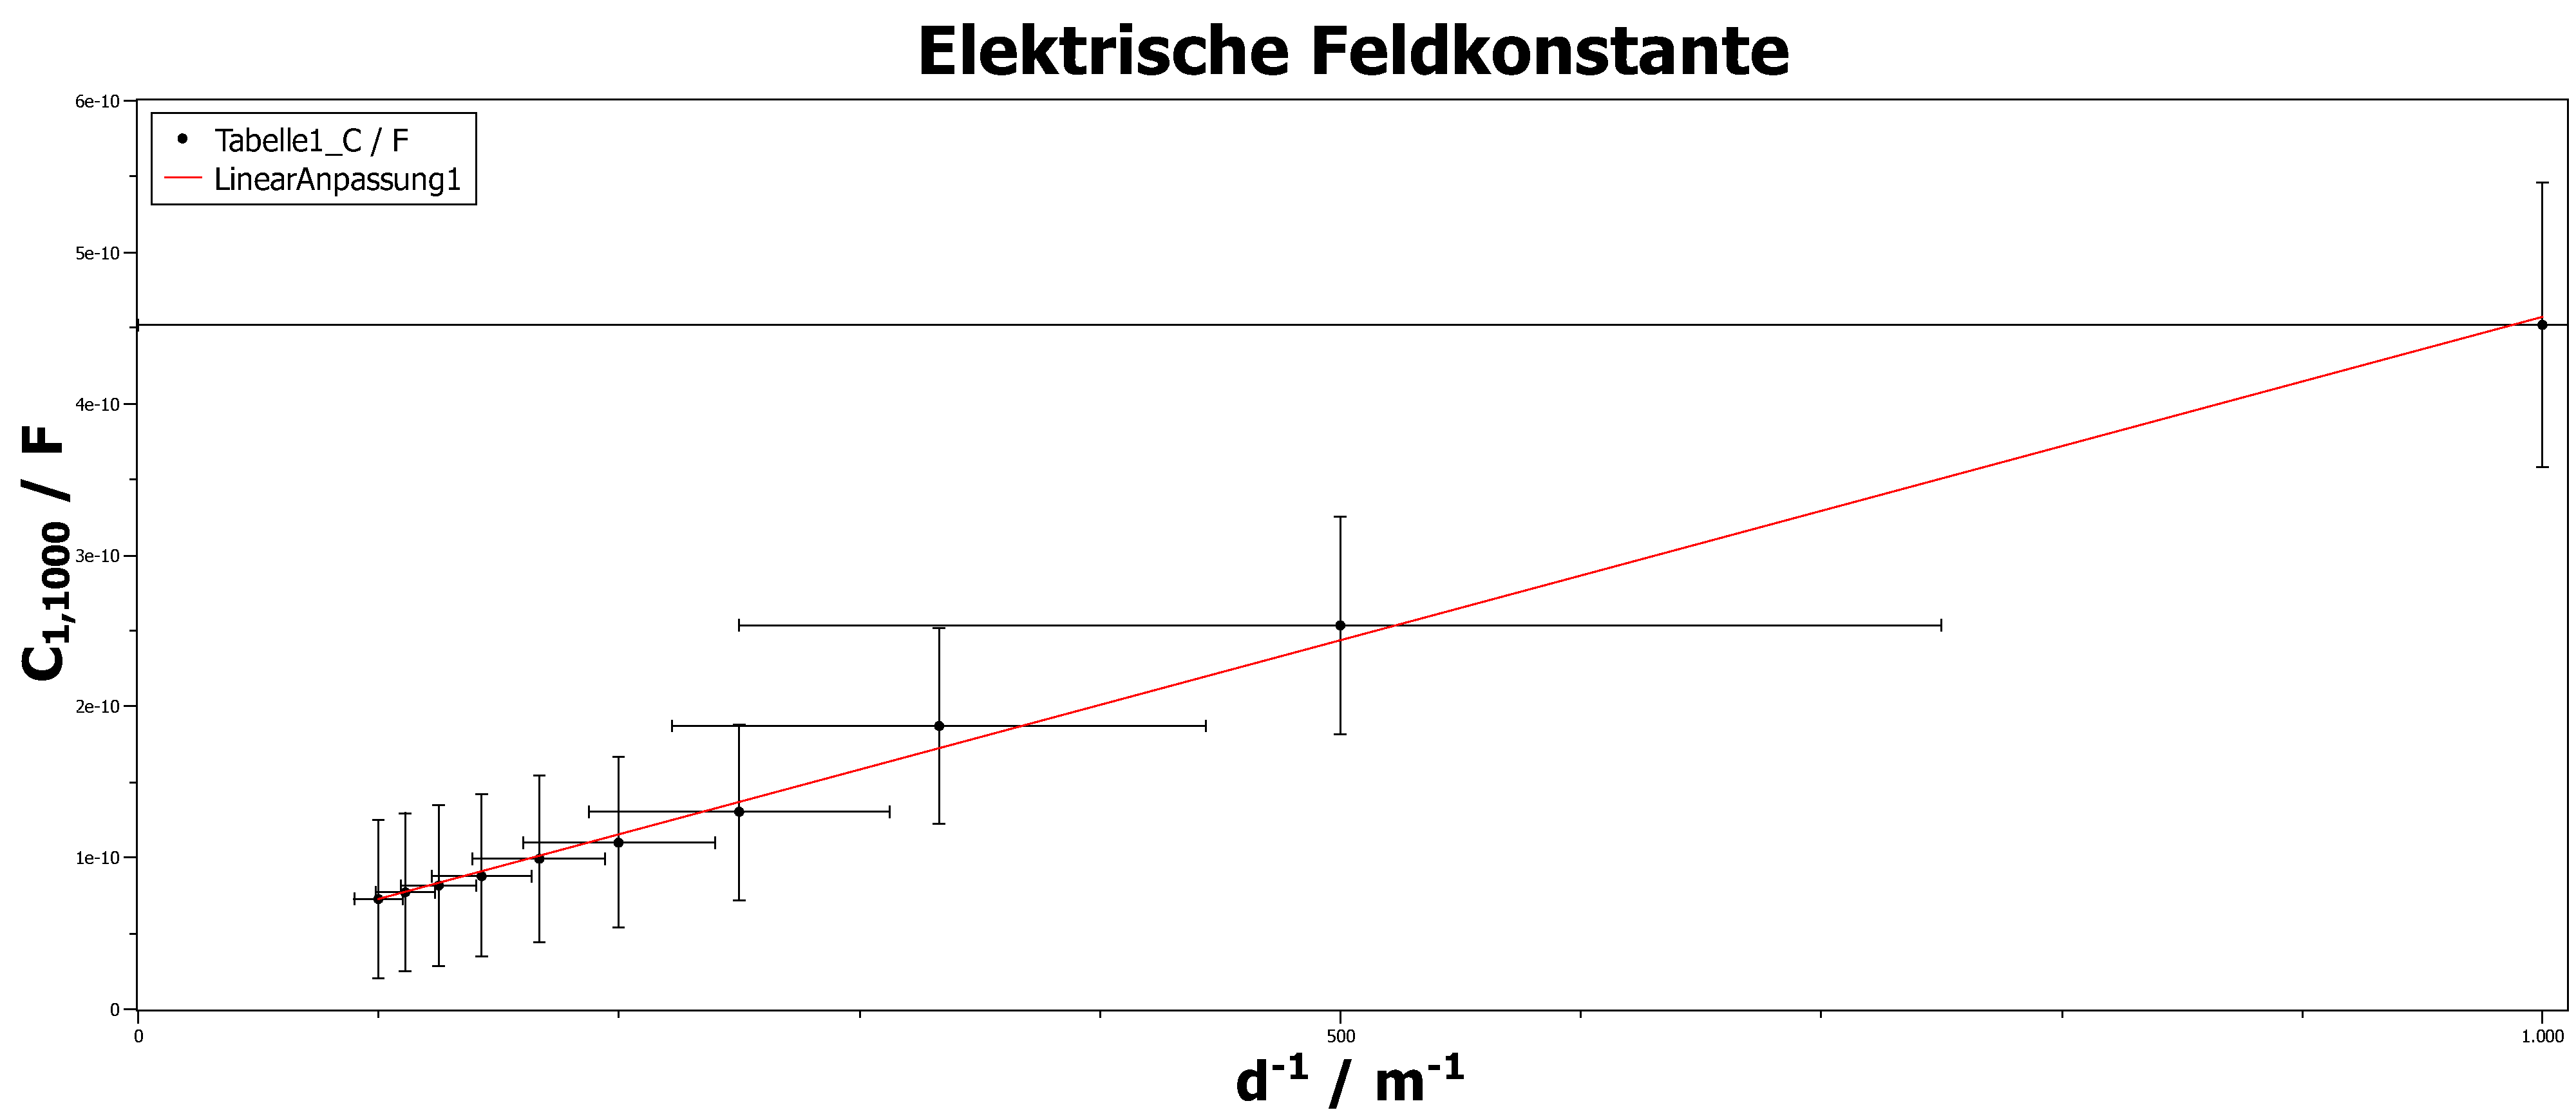
\includegraphics[width=.95\textwidth]{diagramme/Elektrische_Feldkonstante.pdf}
    \caption[Diagram elektrische Feldkonstante]{Diagram elektrische Feldkonstante}
    \label{fig:mu_0}
\end{figure}
%
mit der durch \textit{SciDAVis} ermittelten Steigung der Ausgleichsgeraden von:
%
\begin{align}
    m=(4,3 \pm 0,7){\cdot 10^{-13}\frac{\text{As}\cdot \text{m}}{\text{V}}}
\end{align}
Für die elektrische Feldkonstante $\varepsilon_{0}$ gilt also:
\begin{align}
    \varepsilon_{0} &= \frac{m}{\varepsilon_{R}\cdot A} \nonumber \\
    &= \frac{4,3\SI{}{\cdot 10^{-13} \frac{As \cdot m}{V}}}{ \frac{\pi}{4} \cdot (\SI{0,255}{m})^{2} } \nonumber \\
    &= 8,420\SI{}{\cdot 10^{-12}\frac{As}{Vm}}
\end{align}
%
\subsection{Fehler der experimentell bestimmten elektrischen Feldkonstante}
Der Fehler der elektrischen Feldkonstante hängt von der Abweichung der Steigung und des Durchmessers ab. So gilt:
\begin{align}
    \varepsilon_{0} &= \frac{4 m}{D^{2} \pi} \nonumber \\
    \Delta\varepsilon_{0} &= \left\vert\frac{\partial\varepsilon_{0}}{\partial m}\right\vert \cdot \Delta m + \left\vert\frac{\partial\varepsilon_{0}}{\partial D}\right\vert \cdot \Delta D \nonumber \\
    &= \frac{4}{D^2 \pi} \cdot \Delta m + \frac{8 m}{D^3 \pi} \cdot \Delta D \nonumber \\
    &= \frac{4}{(\SI{0,255}{m})^{2} \cdot \pi} \cdot \SI{0,7}{\cdot 10^{-13}\frac{As\cdot m}{V}} + \frac{8 \cdot \SI{4,3}{\cdot 10^{-13}\frac{As \cdot m}{V}}}{(\SI{0,255}{m})^{3} \cdot \pi} \cdot \SI{0,005}{m} \nonumber \\
    &= \SI{1,37}{\cdot 10^{-12}\frac{As}{Vm}} + \SI{0,33}{\cdot 10^{-12}\frac{As}{Vm}} \nonumber \\
    &= \SI{1,70}{\cdot 10^{-12}\frac{As}{Vm}}
\end{align}
Ermittelte elektrische Feldkonstante:\par
\begin{align}
    \varepsilon_{0}=(8,4\pm 1,7){\cdot 10^{-12}\frac{\text{As}}{\text{Vm}}}
\end{align}
%
%
%
\section{Bestimmung der Dielektrizitätszahlen}
Über das Verhältnis der beiden Kapazitäten mit und ohne Platte kann nach \gl{eq:rel_feld} die Dielektrizitätszahl
$\varepsilon_{r}$ des jeweiligen Materials bestimmt werden.\par
Zunächst wurden in \textit{SciDAVis} die Spannungen $ U_{2} $, so wie die Kapazitäten $ C_{D} $ und $ C_{0} $ umgerechnet
und abschließend in Relation gesetzt. Die so ermittelten Mittelwerte mit jeweiliger Standardabweichung sind folgende:
\begin{align}
    \varepsilon_{R,Plexiglas} &= 4,05\pm 0,15\\
    \varepsilon_{R,Pertinax} &= 8,73\pm 0,92
\end{align}
\chapter{Fazit}
Rückblickend ist zu sagen, dass der Versuch eine gute Möglichkeit ist, den Kondensator näher zu untersuchen. Es ist durch
den Aufbau vergleichsweise einfach, Kapazität, elektrische Feldkonstante und Dielektrika zu ermitteln.\par
Anhand des Diagramms in \bild{fig:farad} ist zu erkennen, dass die drei Messreihen ähnliche Ergebnisse für die Kapazität
geliefert haben. Der tatsächlich berechnete Wert liegt ebenfalls in unmittelbarer Nähe der anderen Punkte. Alle Punkte
werden durch die jeweiligen Fehlerbalken gedeckt. Der größte Teil, der den Fehler ausmacht, ist vermutlich die Spannung
$ U_{2} $, da der Zeiger des Messgerät immer weiter ausgeschlagen hat. Als Abhilfe wurde die Spannung unmittelbar nach
Betätigen des Umschalters abgelesen.\par
Der Fehler des berechneten Kapazitätswerts hängt von der Abweichung des Durchmessers und des Abstandes der Kondensatorplatten
ab. Da der Durchmesser schwer zu messen war, wurde mit $ \Delta D=\SI{0,5}{cm} $ eine relativ hohe Ungenauigkeit gewählt.
Noch höher gewählt wurde die Abstandsungenauigkeit mit $ \Delta d=\SI{1}{mm} $, da die Skala nur auf ein Millimeter genau
abgelesen wurde, jedoch durch die Feinverstellung die Ungenauigkeit viel geringer ist als ein Millimeter.\par
Die Bestimmung der elektrischen Feldkonstante war ebenfalls unkompliziert und führte mit
$ \varepsilon_{0}=(8,4\pm 1,7){\cdot 10^{-12}\frac{\text{As}}{\text{Vm}}} $ zu einem plausiblen Ergebnis. Die Abweichung
deckt sich mit dem Literaturwert für \(\varepsilon_0\) von \( \SI{8,854}{\cdot 10^{-12} \frac{As}{Vm}}\) \cite{Haberle.2007}.
Durch das
Diagramm in \bild{fig:mu_0} ist die Linearität gut zu erkennen. Jedoch erscheinen die Fehlerbalken aufgrund der Fehlerfortpflanzung
mit abnehmendem Abstand sehr groß. Der Fehler der elektrischen Feldkonstante setzt sich zusammen aus der Durchmesserabweichung,
welche nur einen kleinen Teil des Gesamtfehlers ausmacht, und aus dem mit Hilfe von \textit{SciDAVis} ermittelten Fehler
der Steigung \(m\).
Das hängt vermutlich mit dem wie bereits erwähnten und zu hoch gewählten Abstandsfehler zusammen.\par
Die Aufnahme der Messwerte für die Bestimmung der Dielektrizitätszahl war zwar einfach durchzuführen, brachte dennoch einige
kleine Probleme mit sich. Beim Einführen und Herausnehmen der Platten wurde vermutlich der Abstand ein paar Mal
ungewollt verändert, was sich vor allem bei größeren Spannungen $ U_{2} $ beim Pertinax erkenntlich gemacht hat. Das
Ablesen der Spannung $ U_{2} $ wurde durch das Umstellen und Umdenken der Größenordnung am Messgerät erschwert. Als
Ergebnis kamen mit $ \varepsilon_{r,Plexiglas}=4,05\pm 0,15 $ und $ \varepsilon_{r,Pertinax}=8,73\pm 0,92 $ dennoch
Werte mit (relativ) kleinen Abweichungen heraus. Die Mittelwerte und Standartabweichungen der Messreihen in \tabelle{tab:mess2}
verdeutlichen, wie genau die Messungen tatsächlich waren.\par
Trotz kleinerer Probleme ist der Versuch nichts desto trotz gut geeignet für die Behandlung der Komponenten eines
Kondensators und führte zu erwarteten Resultaten.
%-------------------
\newpage
\listoffigures 
\listoftables
\addchap{Verwendete Symbole}
\begin{table}[h]
    \begin{tabular}{@{}ll@{}}
        $A$ & Fläche der Kondensatorplatten\\
        $C$ & Kapazität\\
        $C_0$ & Kapazität des Kondensators mit Luft als Dielektrikum\\
        $C_D$ & Kapazität des Kondensators mit unbekanntem Dielektrikum\\
        $D$ & Durchmesser der Kondensatorplatten\\
        $E$ & Elektrische Feldstärke\\
        $Q$ & Elektrische Ladung \\
        $U$ & Elektrische Spannung\\
        $d$ & Abstand der Kondensatorplatten\\
        $m$ & Steigung im \(C(d^{-1})\)-Diagram\\
        & \\
        $\varepsilon_0$ & Elektrische Feldkonstante\\
        $\varepsilon_r$ & Dielektrizitätszahl\\
    \end{tabular}
    \label{tab:glossar}
\end{table}
\appendix
\chapter{Anhang}
\begin{table}[h]
    \centering
    \caption[Messwerte1]{Messwerte1}
    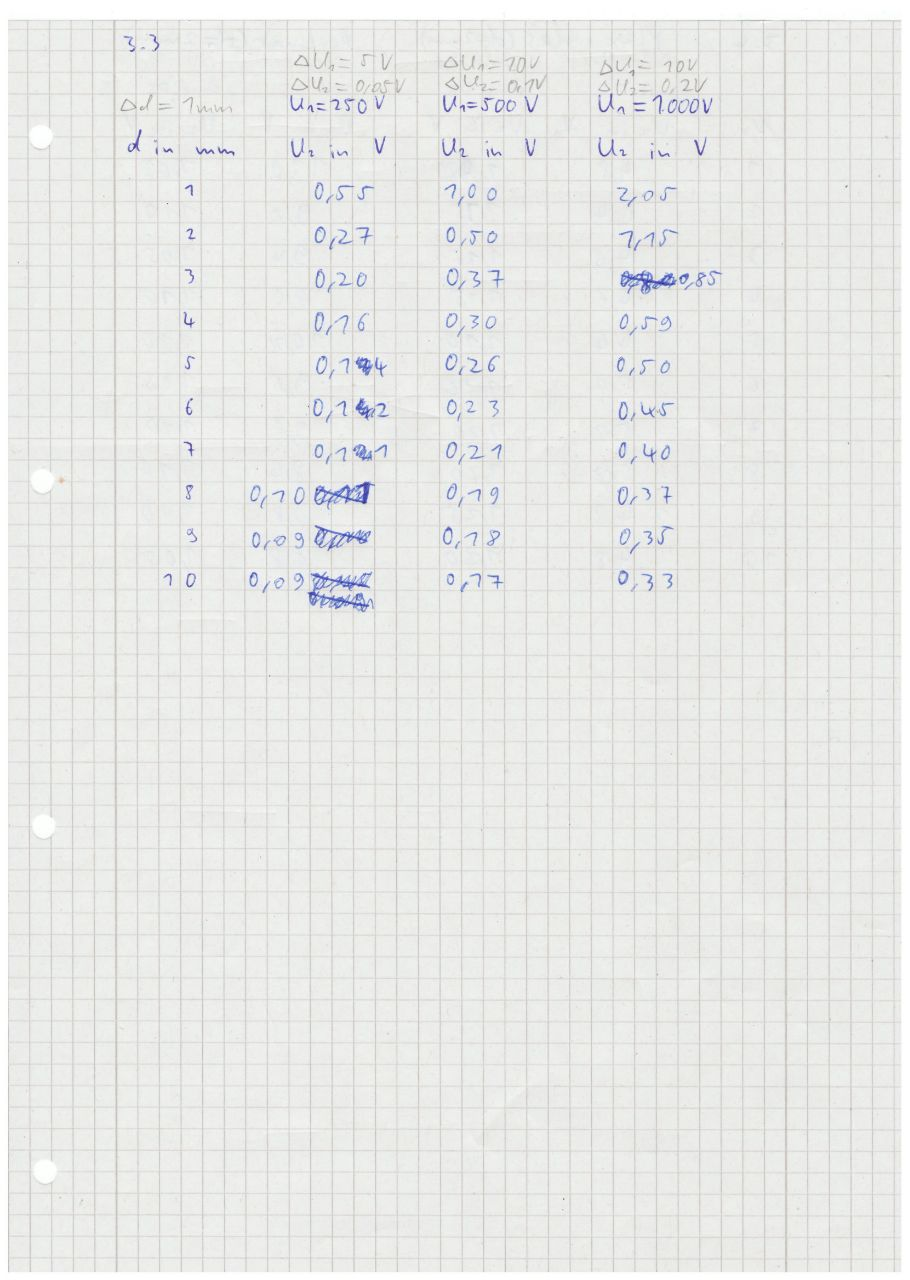
\includegraphics[height=.75\textheight]{messungen/messwerte1.jpg}
    \label{tab:mess1}
\end{table}
%
\begin{table}[h]
    \centering
    \caption[Messwerte2]{Messwerte2}
    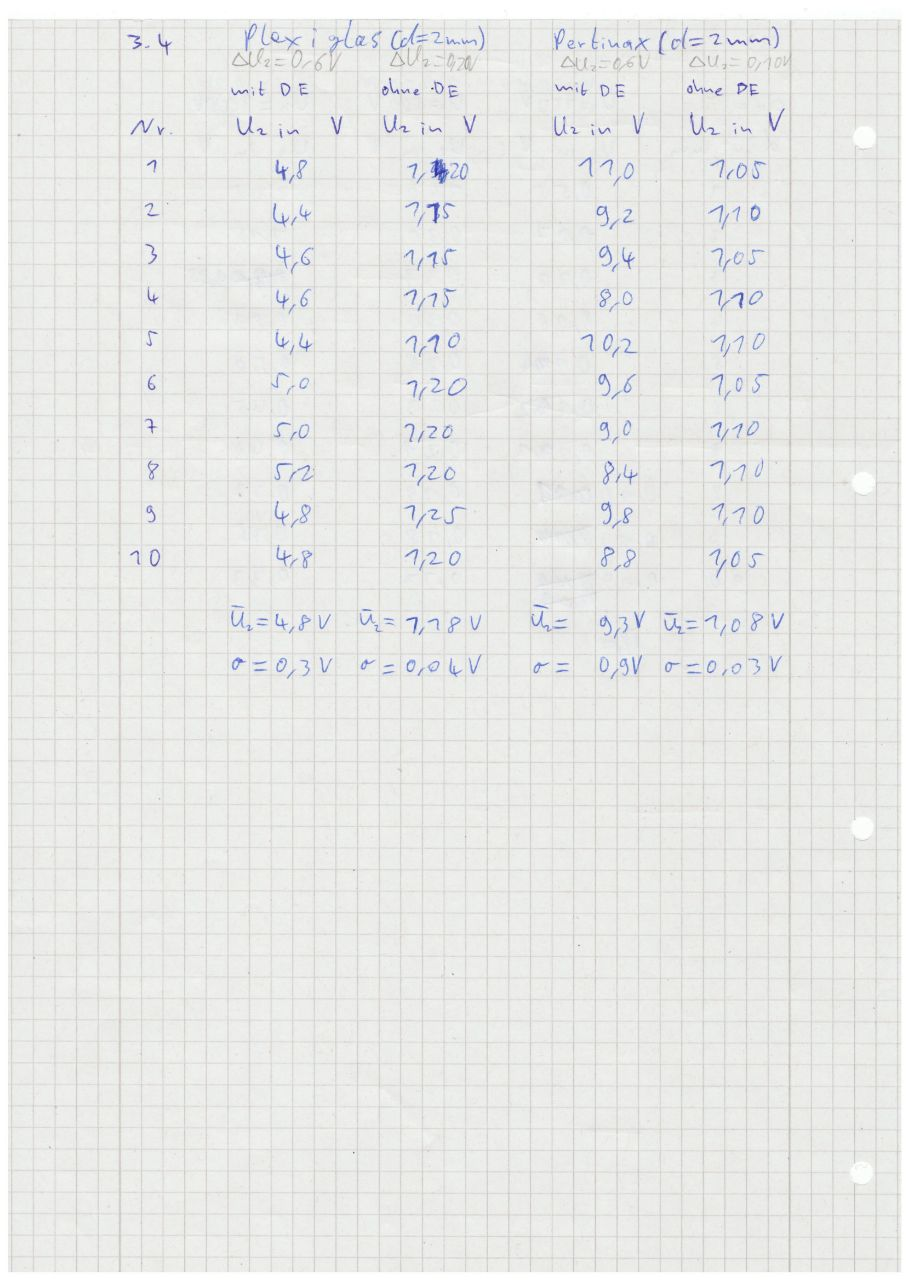
\includegraphics[height=.75\textheight]{messungen/messwerte2.jpg}
    \label{tab:mess2}
\end{table}
\printbibliography
%\bibliographystyle{plaindin}
%==========================================
\end{document}